Virtualization is a way for a data center to reduce cost and power by overcommitting and sharing system resources across disparate operating systems with common hardware.  
In a single server environment or HPC cluster there can be \emph{interference} \cite{paul} or \emph{system noise}\cite{tsafrir} caused by complex software layers (Application, OS, and Hardware), which contributes to poor application performance.  
The hypervisor, as well as multiple external guest virtual machines (Figure \ref{virtStack}), compete for system resources and add to this interference.  
Existing performance tools do not show interference from the hypervisor or external guests.  
System-wide Profiling tools are available on limited platforms, and require significant guest kernel support, configuration, and coordination.  
Additionally, profiling is a great tool for test and development, but may not be a great solution for production systems.
Performance monitoring tools from the virtual guests do not currently provide information about external systems.\\
\textbf{Thesis:  }Sharing resource utilization counters across all layers of virtualization, we can dynamically measure the interference from virtualization and external systems.

%In order to dynamically analyze performance problems from interference we can share system-wide ional layers of virtualization. 

\indent Due to the cost savings and decreased physical administration overhead, Data Centers and Businesses are moving toward virtualized environments.  In 2008 Gartner’s showed that 12\% of hardware at data centers were virtualized, and then predicted that by 2013 61\% would be virtualized \cite{gartners}.   Additionally, research from Ramya and Edwin show tremendous growth in Platform As A Service (PAAS) where an entire system platform is dynamically provisioned in a cloud computing service \cite{ramya}.   Massive data centers are able to provide virtual systems, and manage large clusters of shared resources, for a fraction of the price of building a physical server for each customer.

\indent Since each guest machine only uses a portion of the available resources at any given time, the total resources allocated to all guest VMs can exceed the total physical resources \cite{huber2, amit, buell1}.   This idea of overcommitting resources is the same as preemptive multitasking, where multiple processes share a single CPU; and OS virtual memory, where the total memory available to applications exceeds the physical memory capacity.  In order to maximize resources, IT Data Centers need to overcommit the resources, with the hope that multiple virtual guest machines do not need all resources concurrently.  

\begin{figure}[!h]
  \begin{center}
  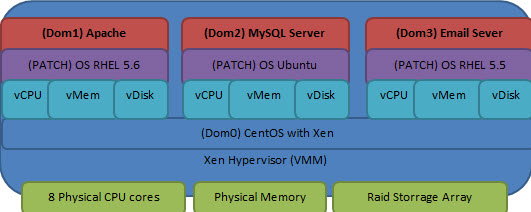
\includegraphics[width=6in]{images/VirtualizationExample.jpg}
  \caption{In this example there are 3 paravirtualized guests (DomU) running on a Xen Server.  The Xen hypervisor and Dom0 divide, share, and overcommit the physical resources between the 3 guest domains.  Each guest has access to virtual resources and not physical hardware.}
  \label{virtStack}
  \end{center}
\end{figure}

\indent This research presents a method for analyzing performance data at runtime in the guests and Virtual Machine Monitor (VMM).   With this framework we can detect the interference cause by virtualization and sharing of resources between multiple guests.  Additionally, we can determine which system resource (memory, CPU, or IO) needs to be modified or is used inefficiently.  This could significantly reduce time spent troubleshooting and analyzing performance problems in virtualized environments.

\indent This project will add the following contributions for virtualization:
\begin{enumerate}
\item Define the layers of abstraction in virtual environments.
\item Define the physical and virtual resources which need to be measured.
\item Examine some common counters, and metrics which can measure resource utilization.
\item Design a framework to collect resource metrics at several layers and quantify the interference from virtualization.
\item Virtualization test suite that causes I/O interference.
\item Example tool which dynamically analyzes runtime interference.
\item Introduce \emph{disk pinning} for virtualization where separate physical disks are assigned to individual virtual servers.
\end{enumerate}

\indent The rest of this document is organized as follows:  In section 2, we review a real problem example in a large data center, and the challenges faced with existing tools.  In section 3, we examine the current state of tools and techniques used to profile and analyze performance issues with virtualization.  Section 4 looks at related works that have identified interference and methods of root cause analysis.  In section 5 we define the needed data and an example tool that can collect and analyze this data.  The last sections are dedicated to the test suite infrastructure to both create the interference and show the accuracy of the analysis.  We also look at possible other uses and what needs further investigation.
